
%%%%%%%%%%%%%%%%%%%%%%% file typeinst.tex %%%%%%%%%%%%%%%%%%%%%%%%%
%
% This is the LaTeX source for the instructions to authors using
% the LaTeX document class 'llncs.cls' for contributions to
% the Lecture Notes in Computer Sciences series.
% http://www.springer.com/lncs       Springer Heidelberg 2006/05/04
%
% It may be used as a template for your own input - copy it
% to a new file with a new name and use it as the basis
% for your article.
%
% NB: the document class 'llncs' has its own and detailed documentation, see
% ftp://ftp.springer.de/data/pubftp/pub/tex/latex/llncs/latex2e/llncsdoc.pdf
%
%%%%%%%%%%%%%%%%%%%%%%%%%%%%%%%%%%%%%%%%%%%%%%%%%%%%%%%%%%%%%%%%%%%


\documentclass[runningheads,a4paper]{llncs}

\usepackage{amssymb}
\setcounter{tocdepth}{3}
\usepackage{graphicx}

\usepackage{url}
\urldef{\mailsa}\path|{alfred.hofmann, ursula.barth, ingrid.haas, frank.holzwarth|
\urldef{\mailsb}\path|anna.kramer, leonie.kunz, christine.reiss, nicole.sator,|
\urldef{\mailsc}\path|erika.siebert-cole, peter.strasser, lncs}@springer.com|    
\newcommand{\keywords}[1]{\par\addvspace\baselineskip
\noindent\keywordname\enspace\ignorespaces#1}

\begin{document}

\mainmatter  % start of an individual contribution

% first the title is needed
\title{Crowdsourcing Enabled Ontology Engineering}
%Alternatives
%* Crowd-based ontology engineering
%* Tool support for crowd-based ontology engineering

% a short form should be given in case it is too long for the running head
\titlerunning{Crowdsourcing Enabled Ontology Engineering}

% the name(s) of the author(s) follow(s) next
%
% NB: Chinese authors should write their first names(s) in front of
% their surnames. This ensures that the names appear correctly in
% the running heads and the author index.
%
\author{Gerhard Wohlgennant
\and Marta Sabou\and X Y}
%
\authorrunning{Wohlgennant et al.}
% (feature abused for this document to repeat the title also on left hand pages)

% the affiliations are given next; don't give your e-mail address
% unless you accept that it will be published
\institute{WU\
Vienna\\
\mailsa\\
\url{http://www.wu.ac.at}}

%
% NB: a more complex sample for affiliations and the mapping to the
% corresponding authors can be found in the file "llncs.dem"
% (search for the string "\mainmatter" where a contribution starts).
% "llncs.dem" accompanies the document class "llncs.cls".
%

%\toctitle{Lecture Notes in Computer Science}
%\tocauthor{Authors' Instructions}
\maketitle


\begin{abstract}
Recent years have seen an increase in the use of crowdsourcing based methods at various stages of the ontology engineering lifecycle (e.g., verification of subsumption, assigning equivalences between concepts etc) thus laying the foundations of a novel approach to ontology engineering. Take up of this early research by the community at large, especially by practitioners, is however currently hampered by 1) a lack of understanding of which stages of the ontology engineering process can be crowdsourced and 2) tool support in ontology engineering platforms that would allow easy insertion of crowdsourcing into ontology engineering workflows. In this paper we perform an overview of recent works in the area and take a scenario-based approach to identifying those stages of the OE process where crowdsourcing makes sense. Then, we present the �uComp Protege plugin�, a plugin for the popular Protege ontology engineering platform that facilitates the integration of crowdsourcing stages into the OE process. TBD: clarify novelty (e.g., which new tasks we introduce?), sum up some important evaluation results.
\keywords{human computation, crowdsourcing, ontology engineering, ontology learning, Protege plugin}
\end{abstract}


\section{Introduction}

RQ1: Which tasks can be crowdsourced? How do they fit in the OE workflow?

RQ2: How to provide tool support for crowdsourcing in OE?



\section{Related Work - MS}

Noy and colleagues [1] focus on the task of verifying subclass-superclass relations that make up the ontology hierarchy. Their main interest is in understanding whether crowdsourcing via MTurk is a viable alternative for this task and therefore they perform a series of experiments that compare microworkers against students, evaluate performance differences over different types of ontologies (e.g., upper ontologies vs. generic ontologies) and finally assess crowd-performance in specialized domains. The paper concludes that micro-workers are a viable alternative for verifying subclass-superclass relations and also introduces a vision for a tool support that would facilitate the integration of crowdsourcing into OE workflows. We present such a tool in this paper, that not only allows the ontology engineer to crowdsource subsumption verification, but also a set of other tasks that often appear in ontology engineering scenarios.


[TBD - table]

\section{Ontology Engineering Scenarios - Ontology Learning - MS}
 (1 or both of the following)
OL - Gerhard�s work on automatic OL from text \& other sources

OR - using the Watson plugin

TBD: Relate to the "Embedded HC paradigm"

\section{Ontology Engineering Tasks for Crowdsourcing - MS}

From the scenarios above as well as the related work, we distinguish a set of generic ontology engineering tasks that are suitable for crowdsourcing and which are likely to be of interest in a wide range of ontology engineering scenarios:

\begin{description}
\item[T1. Verification of Domain Relevance.]  Is a concept/instance relevant for a domain? 
\item[T2. Verification of Relation Correctness.] Does a certain relation between two ontology entities hold? These could be a set of generic relations (sameAs, subClassOf, instanceOf), but also arbitrary named relations to be specified by the ontology engineer. The crowd here would have to vote (yes/no) for a given triple (Subject - Relation - Object). This task is the focus of [1].
\item[T3. Learning of Relation Names.] This is also a very difficult task in OL in general - the workers are presented with two terms and can choose between a set of given relations what applies. These relations can be a set of OWL relations that all ontologies have as well as a (restricted) number of domain specific relations specified by the expert (e.g., �influences�). [BTW, since this is a complex task it could be split up into a sequence of 3 simpler tasks: 1) given two terms workers agree whether these are related or not; 2) those pairs that were judged related are then passed to another task where a correct relation is selected; 3) in the third task, the quality of the relations is checked - practically T2]
Available relation labels are some predefined (like subClassOf) and those from the target ontology (all ObjectProperties) -- if more than 20 .. spread over multiple windows (depending on window size)
Have a limit of 5 relation labels in the Protege interface
All pairs with a certain relation (defined by the user in a text field, eg �relation�) are sent to the uComp API (or directly to CF).
If you want to use just a subset of relations: have a window where you select (checkboxes) the actual pair to be sent.
In CrowdFlower -- also have the choice to add a free text label
output: be able to sort by certainty from CF ..
\end{description}

\section{The uComp Protege Plugin - GW}


% T1. Verification of Domain Relevance.  Is a concept/instance relevant for a domain?
% T2. Verification of Relation Correctness. Does a certain relation between two ontology entities hold? These could be a set of generic relations (sameAs, subClassOf, instanceOf), but also arbitrary named relations to be specified by the ontology engineer. The crowd here would have to vote (yes/no) for a given triple (Subject - Relation - Object). This task is the focus of [1].
% T3. Learning of Relation Names. This is also a very difficult task in OL in general - the workers are presented with two terms and can choose between a set of given relations what applies. These relations can be a set of OWL relations that all ontologies have as well as a (restricted) number of domain specific relations specified by the expert (e.g., ÒinfluencesÓ). [BTW, since this is a complex task it could be split up into a sequence of 3 simpler tasks: 1) given two terms workers agree whether these are related or not; 2) those pairs that were judged related are then passed to another task where a correct relation is selected; 3) in the third task, the quality of the relations is checked - practically T2]

This section describes the actual plugin, ie.~which tasks have been implemented, the features and plugin usage. 
Protege was programmed in Java, it can easily be extended in the form of \emph{plugins} which are typically Java Archive (.jar) files
stored in the Protege plugin directory. The most common form of a Protege plugin is a view plugin, which implements a single view for a specific area of an ontology (e.g. classes, individuals, object properties, \dots).
%Florian: Protege completely was programmed in Java, therefore all plugins also are programmed in Java. Since Protege was developed very modular, it is quite easy to create simply plugins and integrate them into Protege. 
%Florian: All Protege plugins are so called jar-Files (Java Archive), and contains the compiled source code and all needed libraries. The most common form of a Protege plugin is a view plugin, which implements a single view for a specific area of an ontology (e.g. classes, individuals, object properties, ...)

% installation / SETUP 
Installation and setup
* The plugin is available at \url{TODO -- add link once uploaded to Protege}, includes detailed documentation about the tasks and 
the usage of the plugin. TODO (if necessary) documentation is accessible at ..
To use the plugin you need to your uComp-API key\footnote{Request a key from the uComp team, see \ur{http://soc.ecoresearch.net/facebook/election2008/ucomp-quiz-beta/api/v1/documentation/}} in a file named \texttt{ucomp\_api\_key.txt} in folder \texttt{.Protege}.
* Use an existing CF account key .. describe how to use it (place in conf file?!)
%Florian: The CF key has to be associated with the uComp-API key, therefore it has to be communicated to the uComp-API team (see http://soc.ecoresearch.net/facebook/election2008/ucomp-quiz-beta/api/v1/documentation/)
%Florian: The uComp-API key itself must be put into a textfile named "ucomp_api_key.txt" at the users home directory, in the folder ".Protege" (which is created by Protege during installation on both Windows and Linux plattforms) 

% PERSISTENCE 
 All data collected by the plugin which should be persistent is stored in the ontology in \texttt{rdfs:comment} fields,
for example information about the domain, the job ID, and results from the game.
%Florian: all information about the task is stored (depends on the kind of task): domain, validation of whole subtree going on?, additional information, sent to crowdflower or ucomp-quiz, ucomp-api job-id, ...

% give an example SCREEENSHOT with a quick introduction 
\begin{figure*}[htb]
\centering
{\centering \resizebox*{1.0\textwidth}{!}{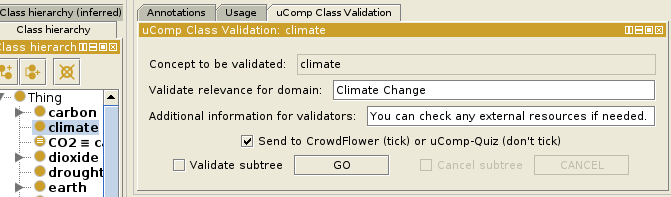
\includegraphics{images/c_rel_check_start.png}}}
 \caption{\label{fig:screen_cr}Screenshot showing the interface for validating a concept.}
\end{figure*}

Figure~\ref{fig:screen_cr} shows the basic interface for the domain relevance task, the other tasks
have similar interface.
Initially, the user adds the new view in the Protege window. The plugin interface contains 
task specific information (eg. the concept selected by the user for validation), 
generic information such as the \emph{domain} of the ontology and \emph{additional information} (see below),
and a \texttt{GO} button start the validation process.


% The common PROCESS 
The process itself is similar for all types of evaluation: (i) the user selects which part of the ontology 
should be verified (eg. a specific concept or all concepts), (ii) a requested is sent to the uComp API, 
(iii) as soon as available, the uComp API presents the results and saves them in the ontology.


% COMMON FIELDS in the UI: domain and additional information
What is common among all tasks handled by the plugin, is the selection of a ``domain'' and that the user can provide
additional information about the task. The domain is simply the field of knowledge which the ontology covers. If entered
once, the domain will be stored in the ontology (as \texttt{rdfs:comment}) and be pre-filled subsequently, but it can also be changed at any time.
For every task, the plugin contains a predefined task description (typically including examples) which is presented to the HC user.
If the ontology engineer wants to extend this task description, he or she can provide more guidelines 
in the field ``additional information''.
TODO: a few words about: validate subtree (only for tasks: concept relevance, subtree validation, TODO)
%Florian: domain will be stored as rdfs:comment in the head of the ontology


% USAGE 
In a nutshell, the user selects the part of the ontology to validate and optinally gives some additional information (see below). 
The plugin sends the request to the HC API (uComp API), which delegates the task to a GWAP or CrowdFlower. 
After enough HC users given their input on the task, the results are sent back to the plugin, which then displays them to the Protégé user. Depending on the result, the user can perform further actions like deleting negatively validated parts of the ontology.
* Explain: With plugins to Protege --> typically additional options in the Windows->Views Menu. 
  So in general, first open an ontology, then select the part of the ontology to verify (eg. the ``classes''), and finally 
  added the verfication frame via the Windows->Views menu.


% TODO -- describe TASKs
Task 1 - Verification of Domain Relevance.
* Being in class view, select the "uComp Class Validation" from the Windows->Views menu. 

into Windows->Views->class view. Add the 


%\section{The �uComp� Protege Plugin - GW}
%
%(not sure what would be the best name for it :))
%describes which of the tasks above are implemented and how + other technical details.

\section{Evaluation}

\subsection{Evaluation Goal}
The goal of the evaluation is to assess the improvements that the uComp Plugin could enable in a typical ontology engineering scenario in terms of typical project completion aspects such as time, cost and quality of output. The usability of the plugin is an additional criteria that should be evaluated. Concretely, our evaluation goals can be summarised into the following questions:

\begin{description}
\item[Time] \textit{How does the use of the plugin affect the time needed to perform ontology engineering tasks?} - We distinguish here the total task time (Ttt) as the time taken from the start of the ontology engineering task until its finalisation; and the time of the ontology engineer spent actively in the task (Toe). In a crowdsourced scenario, Toe < Ttt, because the ontology engineer is only actively working during the outsourcing of the task and the review of the result. In contrast, in a traditional scenario Toe = Ttt. What is of interest to us is the time reduction ratio, that is (Ttt-Toe)/Ttt. (this will be computed as an average over multiple measurements, and over various ontology engineering tasks).

\item[Cost] \textit{Are there cost benefits associated with the use of the plugin?}  We compute costs related to payments for the involved work-force, that is payments to ontology experts and payments to crowd-workers. Costs of ontology experts are computed by multiplying the time they spend on the task (Toe) with an average salary. In order to allow comparison to other similar cost-focused studies [1], the wage of a research scientist was assumed to be \$54,000 per annum.

\item[Quaility] \textit{What are the implications on the quality of the resulting output when using the Plugin?} Several earlier studies [e.g., Thalhammer�13, Sabou�13, Noy?, Sabou�13] have shown that the quality of the semantic tasks performed by crowd-workers is in general similar to (or even better than) the quality of tasks performed by ontology engineers. While the quality of the obtained data is not the core focus of our evaluation, we expect to obtain results similar to those already published [TBD: note however, that unlike earlier studies which focus on simple, atomic tasks, we focus on more complex engineering tasks - is this really true?]

\item[Usability] \textit{Is the plugin usable?} As any end-user tools, the plugin should be easy to understand and use by the average ontology engineer already familiar with the Protege environment.
\end{description}

\subsection{Evaluation Setup}

The setup involves working with two groups of ontology engineers, which will perform the same OE  tasks. 

\subsubsection{Evaluators}

Victims: Adrian, J�rgen (? knows the tool), 2 guys from TU Vienna (Olger, Fajar)
Non-Protege victims: Stefan, Matyas, Michael, Philipp, Heinz, Max G�bel

\begin{description}
\item[Group 1]  This group will make use of traditional (that is manual) methods to perform the three OE tasks. The group consists of X ontology engineers.
\item[Group 2] This group, consisting of Y ontology engineers,  will use the Plugin to perform the three OE tasks. Group 2 will be provided a short tutorial about the plugin (30 minutes) and will have to perform a usability questionnaire about the plugin.
\end{description}

\subsubsection{Evaluation Data}
The input to all evaluation tasks are ontologies generated by an ontology learning algorithm from textual sources. 

For every ontology snapshot, ie. every result of an ontology learning stage, as well as the resulting ontology the system exports an OWL file (using the Turtle seralization format, which can be converted to RDF/XML easily).
The conversion of our internal format for lightweight ontologies is straightforward for concepts (which resemble to OWL classes). WordNet hyper- and hyponym relations are mapped to the OWL subClassOf property. The only challenging aspect is the representation of unlabeled relations in OWL. Our system creates ObjectProperties named "relation\_n", where "n" is an auto-incrementing number, as it is not possible to use the same ObjectProperty more than once. The label for those relations is plainly "relation". The periodically created versions of the domain ontology can be uploaded to a triple store and are thereby accessible via the SPARQL.

We evaluate the plugin over two ontologies covering two diverse domains. Some details of the input ontologies are:

\begin{table}
%\footnotesize

\center
\begin{tabular}{|l|l|c|} \hline
&\textbf{Climate Change Ontology}&\textbf{Finance Ontology}\\ \hline


\textbf{Nr. of Classes} &  &  \\ \hline
\textbf{Nr. of Relations} &  &  \\ \hline
\textbf{Nr. of IsA Relations} &  &  \\ \hline
\textbf{Nr. of Un-named Relations} &  &  \\ \hline

\end{tabular}
\caption{Overview of the ontologies used in the experiments.}
  \label{table:surveygwaps}
  \end{table}


\subsubsection{Evaluation Tasks}
We perform the evaluation of the plugin over three different ontology engineering tasks in order to 1) test different functionalities of the plugin; 2) obtain evaluation result over a range of tasks.

Both user groups will perform the following tasks:

\begin{description}
\item[Task 1: Check concept relevance for a domain] For each concept of the ontology decide whether it is relevant for the domain in question (in our case, climate change). Input: concept and domain name; Output: Y/N ratings -- use a relevant\_to\_domain property -- domain experts use �Y/N�

\item[Task 2: Check the correctness of isA relations] For all isA relations verify whether they are correct, that is a generic/specific relation exists between the domain and range of the relation. Manual experts change the value for a certain annotation property (...\_subClass\_validation\_result)
\end{description}

\subsubsection{Evaluation Metrics}

For time:
For each participant measure Toe, and Ttt, for each task.
Compute averages per participant
Compute group averages and differences
 
For costs:
Compute avg costs per participant and per group and differences
 
For quality: Since we do not have a baseline, we will proceed as follows:
Task 1: compute pair-wise inter-expert agreement for both groups; and between groups � this will measure how different the output is between the plugin and non-plugin group. If it is small then the results are similar; Compute also Cohen�s Kappa
Task 2: same approach as with Task 1
Task 3: Here I think we should evaluate the quality of labels ourselves (em and Gerhard) for each produced ontology; and then  compute a precision value


\end{document}
